\documentclass[conference]{IEEEtran}

\usepackage{verbatim}
\usepackage{framed}
\usepackage{url}
\usepackage{flushend}
\usepackage{multirow}
\usepackage{graphicx}

\newcommand{\codeinline}[1]{{\fontsize{8}{0}\selectfont\texttt{#1}}}
\newcommand{\codeintable}[1]{{\fontsize{6.215}{7.458}\selectfont\texttt{#1}}}
\newcommand{\codefile}[1]{
  \begin{framed}
  \fontsize{5.65}{6.78}\selectfont
  \verbatiminput{#1}
  \end{framed}
}

\begin{document}

\title{CSE6339 -- The Big Assignment\vspace{-14pt}}
\author{Yasser Gonzalez-Fernandez -- ygf@yorku.ca, ygonzalezfernanez@gmail.com\vspace{4pt} \\ March, 2014}

\maketitle


\begin{abstract}
Solutions to the second assignment of the course CSE6339 3.0 Introduction to 
Computational Linguistics. Instructor: Prof. Nick Cercone, Department of 
Electrical Engineering \& Computer Science, York University, Canada.
\end{abstract}

\section{Introduction}


\section{Program Documentation}


\section{Solutions}

\subsection{Problem 1a}

\begin{quote}
``Simulate the straightforward monkey problem. Let the program run long enough to 
give a meaningful estimate of the yield of words. The result will provide a 
useful comparison with later forms of the problem.''
\end{quote}

...the first book of each author listed in Table~\ref{tab:data} (books numbered~1, 
3, 4, 5, 6, 10, 11, 12, 14, 15, 19, 22, 23, 25, and 27)

\codefile{problem1a.py}

\begin{table}
\caption{Relative word yield of the straightforward monkey problem.\label{tab:problem1a}}
\vspace{-10pt}
\begin{center}
\begin{tabular}{cccc}
\hline
Book No. & Avg. Rate & Book No. & Avg. Rate \\
\hline
1  & 14.97\% & 14 & 7.88\% \\
3  & 26.55\% & 15 & 31.49\% \\
4  & 19.51\% & 19 & 34.18\% \\
5  & 31.02\% & 22 & 26.17\% \\
6  & 26.28\% & 23 & 14.91\% \\
10 & 25.13\% & 25 & 11.87\% \\
11 & 18.81\% & 27 & 13.91\% \\
12 & 17.71\% & & \\
\hline
\end{tabular}
\end{center}
\end{table}


\subsection{Problem 1b}

\begin{quote}
``Use the data in Table~\ref{tab:hamlet} to simulate the first-order monkey problem. 
Again let the program run long enough to give a meaningful estimate of the yield 
of words to permit comparison with other results on relative word yield. Try running
this simulation program against other corpora.''
\end{quote}

\begin{table}
\caption{\hspace{2em}Character Distribution from Act III of Hamlet. \newline
Note: 35,224 characters, a small corpus.\label{tab:hamlet}}
\vspace{-10pt}
\begin{center}
\begin{tabular}{crcrcr}
\hline
Char. & Freq. & Char. & Freq. & Char. & Freq. \\
\hline
space & 6,934  & r     & 1,593  & p     & 433   \\
e     & 3,277  & l     & 1,238  & b     & 410   \\
o     & 2,578  & d     & 1,099  & v     & 309   \\
t     & 2,557  & u     & 1,014  & k     & 255   \\
a     & 2,043  & m     & 889   & '     & 203   \\
s     & 1,856  & y     & 783   & j     & 34    \\
h     & 1,773  & f     & 629   & q     & 27    \\
n     & 1,741  & c     & 584   & x     & 21    \\
i     & 1,736  & g     & 478   & z     & 14    \\
\hline
\end{tabular}
\end{center}
\end{table}

\codefile{problem1b.py}

\begin{table}
\caption{Relative word yield of the first-order monkey problem \newline
with the character frequencies in Table~\ref{tab:hamlet}.\label{tab:problem1b}}
\vspace{-10pt}
\begin{center}
\begin{tabular}{cccc}
\hline
Book No. & Avg. Rate & Book No. & Avg. Rate \\
\hline
1  & 15.01\% & 14 & 7.89\% \\
3  & 22.35\% & 15 & 23.46\% \\
4  & 15.31\% & 19 & 24.94\% \\
5  & 23.50\% & 22 & 19.50\% \\
6  & 21.01\% & 23 & 14.68\% \\
10 & 21.89\% & 25 & 12.37\% \\
11 & 18.67\% & 27 & 17.40\% \\
12 & 15.51\% & & \\
\hline
\end{tabular}
\end{center}
\end{table}


\subsection{Problem 1c}

\begin{quote}
``Use the data supplied, data listed in Table~\ref{tab:data}, to simulate the 
second-order and third-order Bronte monkey problem. Again let the program run 
long enough to give a meaningful estimate of the yield of words to permit 
comparison with other results on relative word yield. Try running this 
simulation program against other authors listed.''
\end{quote}

\begin{table}
\caption{Data made available for this assignment.\label{tab:data}}
\vspace{-18pt}
\begin{center}
\begin{tabular}{r@{\hspace{1.1em}}l@{\hspace{1.1em}}l@{\hspace{0.75em}}r}
\hline
No. & Author & Title & Chars. \\
\hline
1  & C. Dickens & A Christmas Carol & 168,925 \\
2  & C. Dickens & A Tale of Two Cities & 773,928 \\
3  & E. Bronte & Wuthering Heights & 662,869 \\
4  & A. Bronte & Agnes Grey & 384,300 \\
5  & C. Bronte & Jane Eyre & 1,051,336 \\
6  & E. R. Burroughs & Tarzan of the Apes & 492,783 \\
7  & E. R. Burroughs & Warlord of Mars & 319,854 \\
8  & E. R. Burroughs & The People that Time Forgot & 212,736 \\
9  & E. R. Burroughs & The Land that Time Forgot & 205,762 \\
10 & H. R. Haggard & King Solomon's Mines & 454,437 \\
11 & J. Cleland & Fanny Hill & 474,725 \\
12 & L. Carroll & Alice's Adventures in Wonderland & 148,580 \\
13 & L. Carroll & Through the Looking Glass & 167,015 \\
14 & W. Irving & Legend of Sleepy Hollow & 69,164 \\
15 & Sir A. C. Doyle & The Adventures of Sherlock Holmes & 575,574 \\
16 & Sir A. C. Doyle & The Lost World & 432,766 \\
17 & Sir A. C. Doyle & The Hound of the Baskervilles & 327,348 \\
18 & Sir A. C. Doyle & Tales of Terror and Mystery & 421,264 \\
19 & M. Twain & Adventures of Huckleberry Finn & 578,345 \\
20 & M. Twain & The Adventures of Tom Sawyer & 397,076 \\
21 & M. Twain & A Connecticut Yankee in & 657,430 \\
   &          & King Arthur's Court & \\
22 & N. Machiavelli & The Prince & 286,854 \\
23 & H. G. Wells & War of the Worlds & 346,458 \\
24 & H. G. Wells & The Time Machine & 182,881 \\
25 & F. Kafka & Metamorphosis & 122,139 \\
26 & F. Kafka & The Trial & 462,372 \\
27 & R. Kipling & The Jungle Book & 279,771 \\
\hline
\end{tabular}
\end{center}
\end{table}

...the books written by the Bronte sisters in Table~\ref{tab:data}
(books numbered 3, 4, and 5).

\codefile{problem1c.py}

\begin{table}
\caption{Relative word yield of the second-order (2nd) and 
third-order (3rd) Bronte monkey problem.\label{tab:problem1c}}
\vspace{-10pt}
\begin{center}

\begin{tabular}{cccccr}
\hline 
\multirow{2}{*}{Book No.} & \multicolumn{2}{c}{Avg. Rate} & \multirow{2}{*}{Book No.} & \multicolumn{2}{c}{Avg. Rate} \\
\cline{2-3} \cline{5-6} 
 & 2nd & 3rd &  & 2nd & 3rd\hspace{0.75em} \\
\hline
1  & 24.78\% & 40.03\% & 14 & 18.57\% & 37.56\% \\
3  & 32.43\% & 44.57\% & 15 & 30.65\% & 41.72\% \\
4  & 27.70\% & 41.87\% & 19 & 35.89\% & 45.42\% \\
5  & 35.38\% & 45.97\% & 22 & 28.89\% & 40.63\% \\
6  & 29.42\% & 41.20\% & 23 & 26.02\% & 40.65\% \\
10 & 30.33\% & 42.09\% & 25 & 23.02\% & 38.12\% \\
11 & 26.16\% & 41.41\% & 27 & 26.94\% & 41.13\% \\
12 & 24.93\% & 38.88\% &    &    & \\
\hline
\end{tabular}
\end{center}
\end{table}


\subsection{Problem 1d}

\begin{quote}
``Investigate the effects of resolution on monkey literacy in the simulation. 
For example round off the matrix elements to the smallest number of places --
or use an equivalent means to reduce the number of keys on the typewriters.''
\end{quote}

...a book of medium size was selected among the books listed in Table~\ref{tab:data} 
(book number 4).

\codefile{problem1d.py}

Fig.~\ref{fig:problem1d} shows the results of the study.

\begin{figure}[!t]
\centering
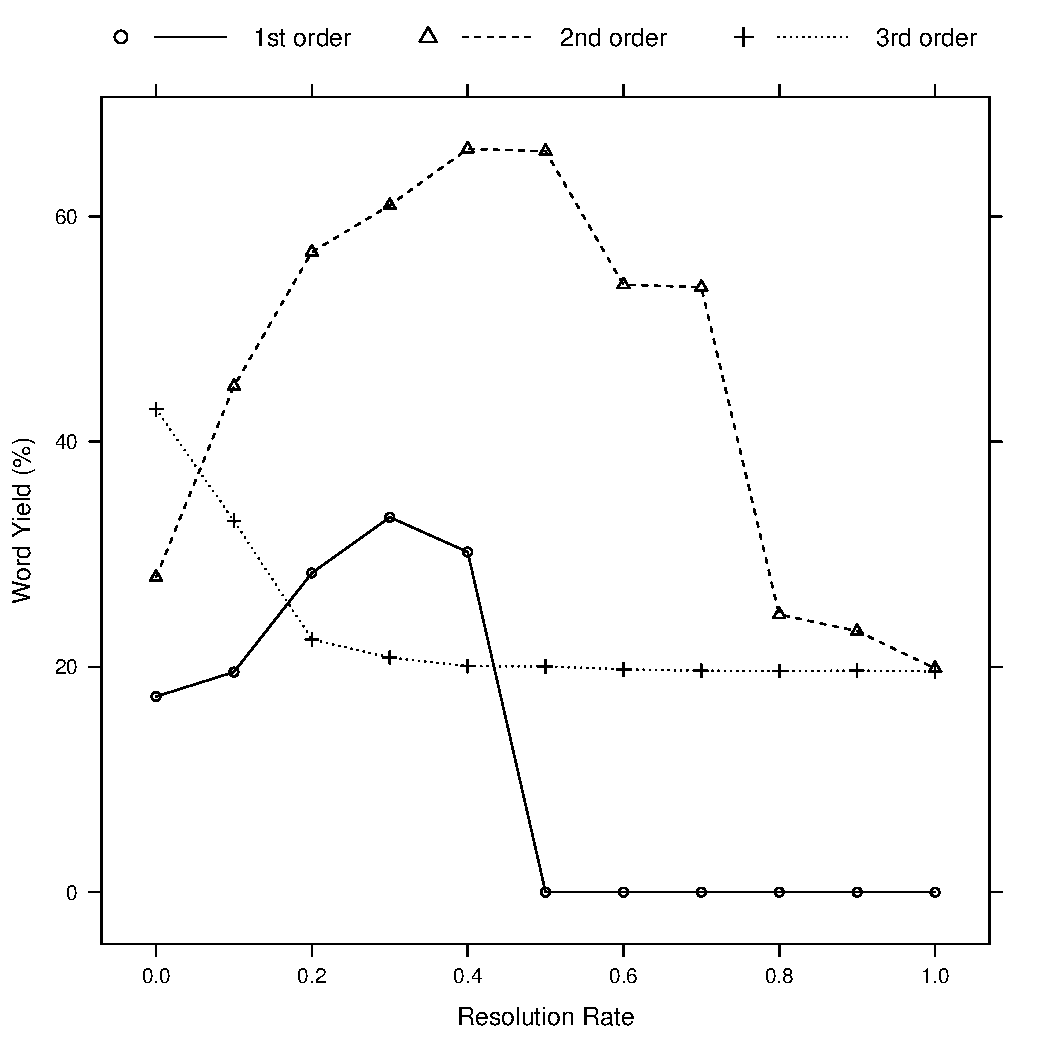
\includegraphics[width=3.4in]{problem1d}
\caption{Effect of resolution on monkey literacy.}
\label{fig:problem1d}
\end{figure}


\subsection{Problem 1e}

\begin{quote}
``Write a routine to compute correlation matrices of the type shown in the 
handout~\cite{Bennett1976} from data supplied (the books shown in Table~\ref{tab:data}).''
\end{quote}

\codefile{problem1e.py}

Figs.~\ref{fig:agnes_grey_2nd_order} and~\ref{fig:agnes_grey_3rd_order} show the results.

\begin{figure}[!t]
\centering
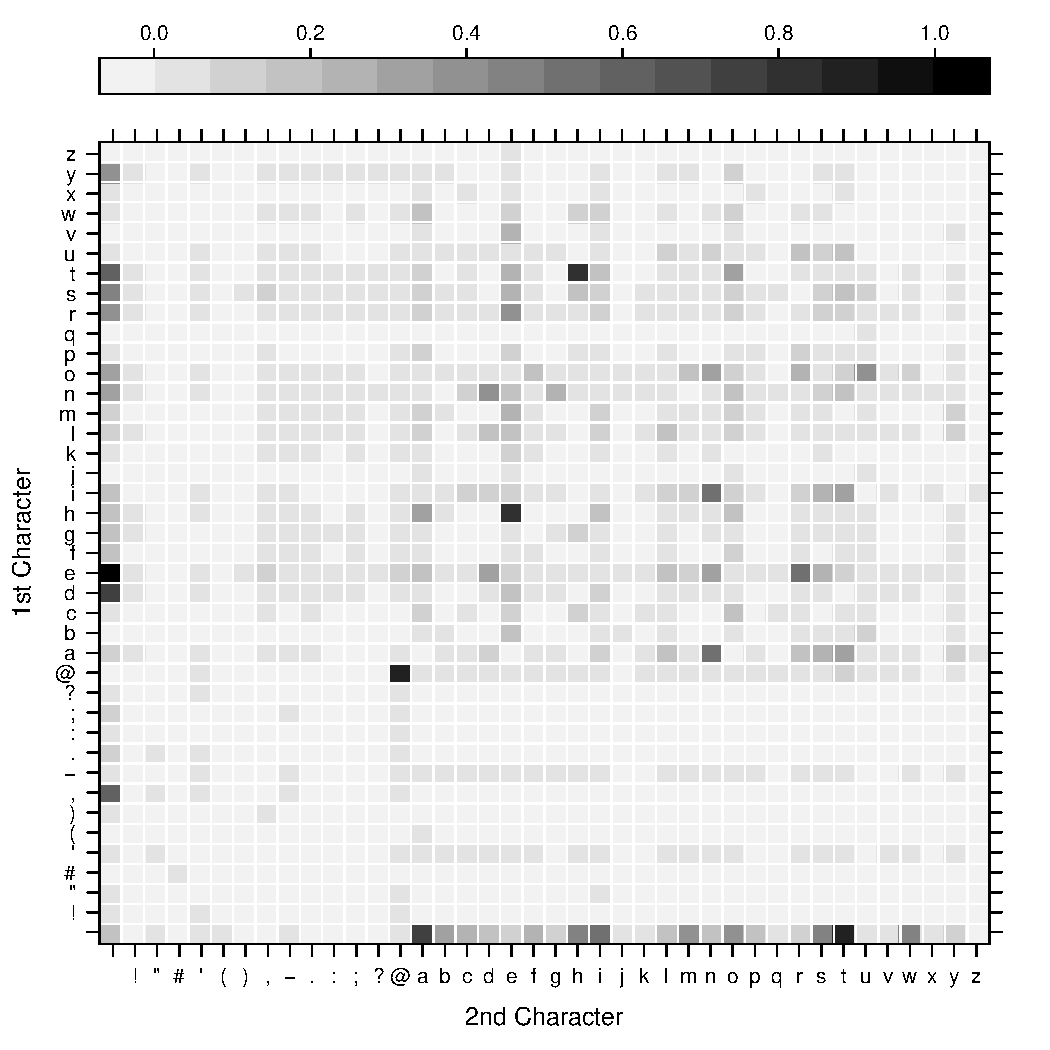
\includegraphics[width=3.4in]{agnes_grey_2nd_order}
\caption{Second-order correlation matrix built from A.~Bronte's `Agnes Grey'.}
\label{fig:agnes_grey_2nd_order}
\end{figure}

\begin{figure*}[!t]
\centering
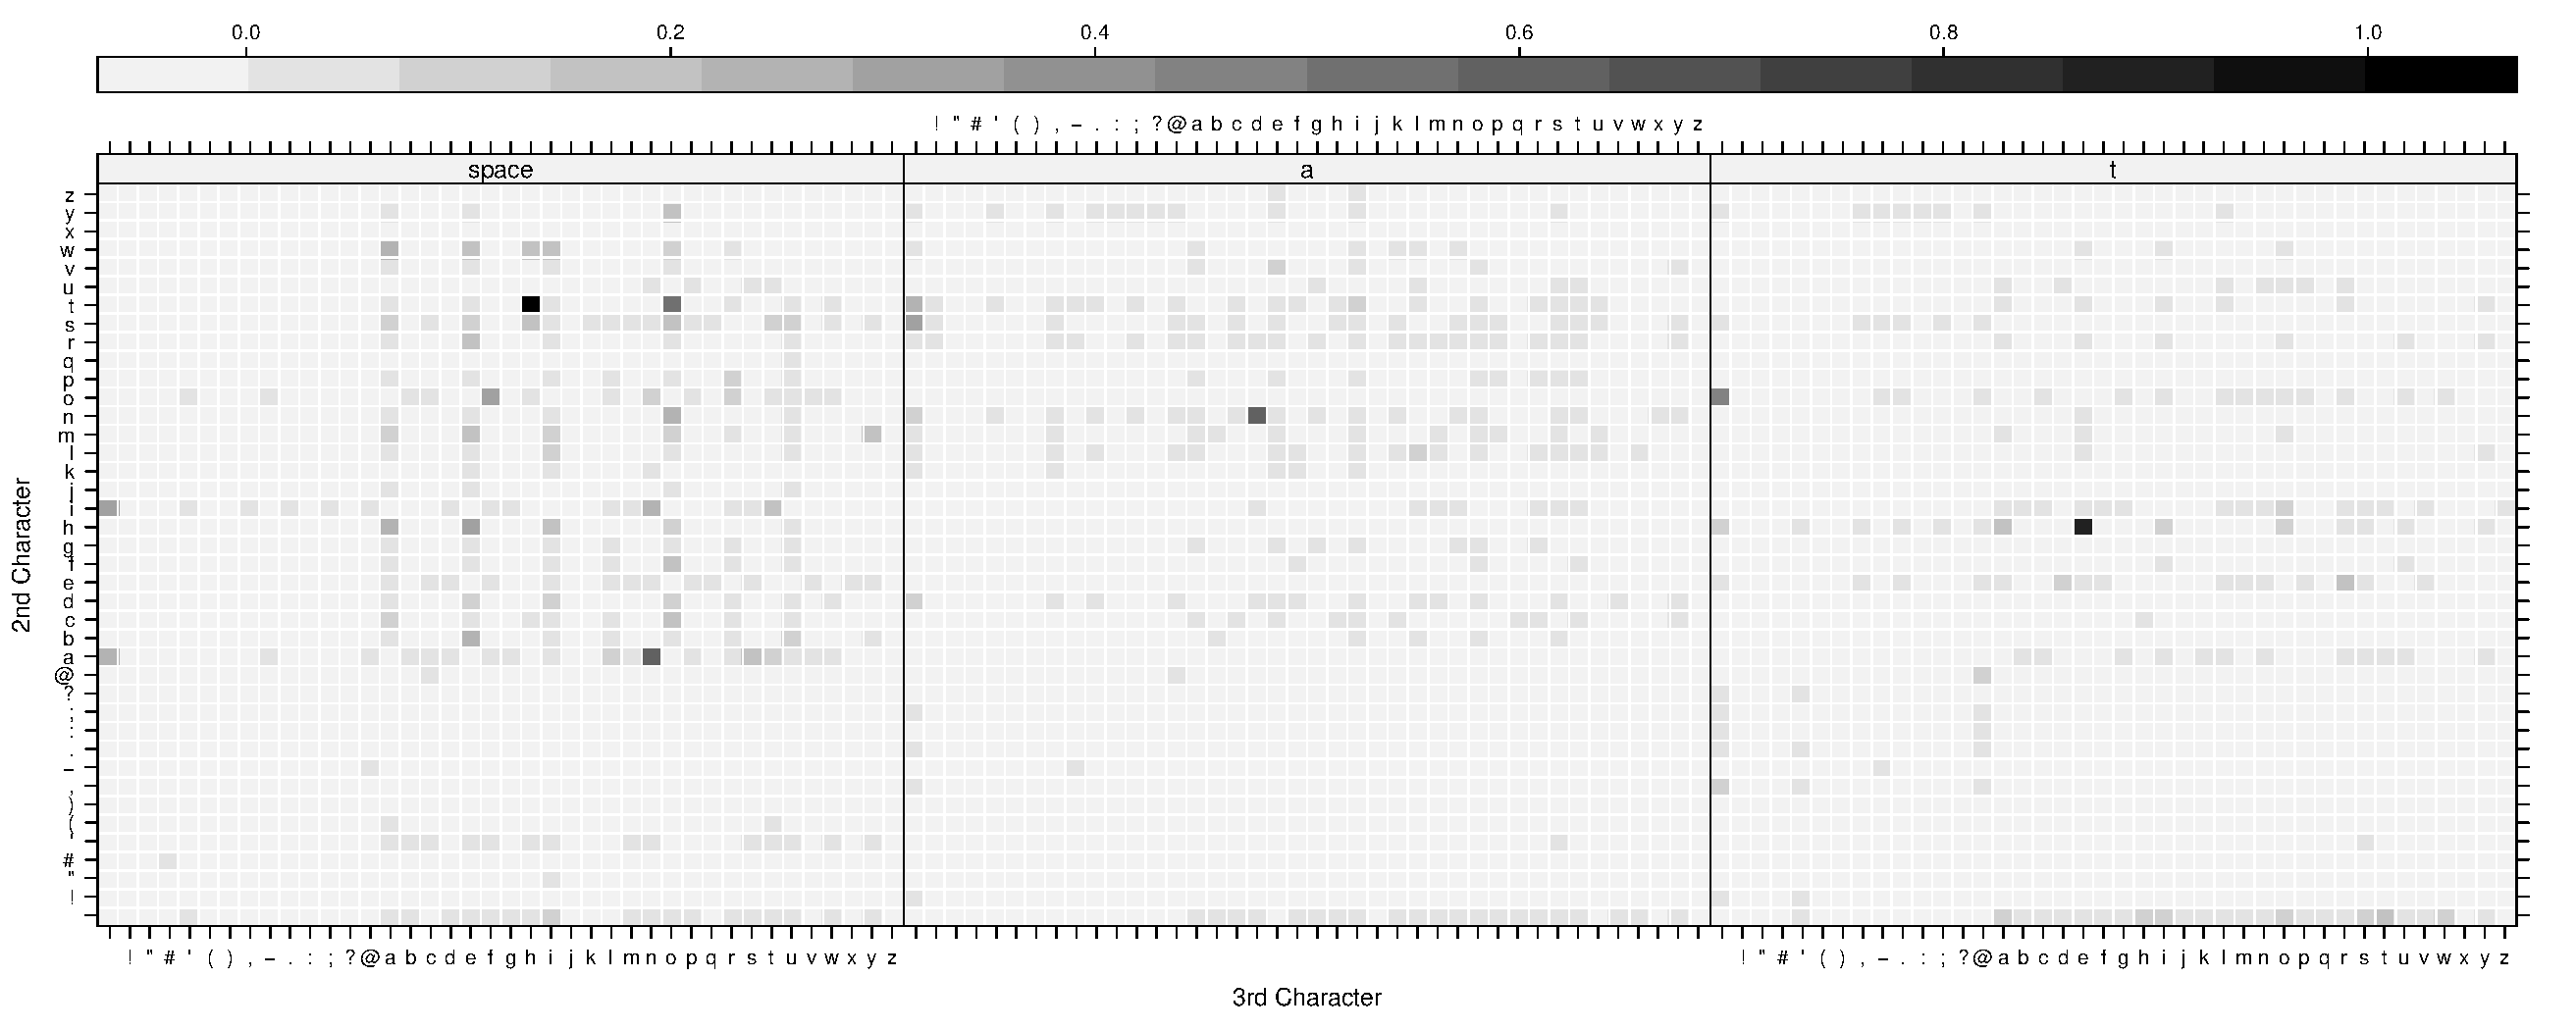
\includegraphics[width=0.9\textwidth]{agnes_grey_3rd_order}
\caption{Selected entries of the third-order correlation matrix built from 
A.~Bronte's `Agnes Grey'. From left to right and top to bottom, the 
panels correspond to trigraphs beginning with the characters space, \codeinline{a},
\codeinline{e}, \codeinline{h}, \codeinline{i}, and \codeinline{t}, respectively.}
\label{fig:agnes_grey_3rd_order}
\end{figure*}

\subsection{Problem 1f}

\begin{quote}
``Using the algorithm in the handout~\cite{Bennett1976} with the pair-correlation matrix 
generated from Irving (book shown in Table~\ref{tab:data}), compute the most 
probable digraph path, which starts with the letter `t'. Compare the result with 
that given in the handout for Poe's `The Gold Bug'''.
\end{quote}

\codefile{problem1f.py}

The book `Legend of Sleepy Hollow' by W. Irving (book number 14 in Table~\ref{tab:data}).
The most probable digraph is \codeinline{the andis,@wofry."bulmpk!-cq} and the 
trigraph \codeinline{the somplack,@}.

The most probable digraph path in Poe's `The Gold Bug' is: \codeinline{the andisouryplf'bj}.

\begin{table}
\caption{\hspace{2em}Most probable digraph (beginning with `t') and \newline 
trigraph (beginning with `th') paths.\label{tab:problem1f}}
\vspace{-10pt}
\begin{center}
\begin{tabular}{cll}
\hline 
\multirow{2}{*}{Book No.} & \multicolumn{2}{c}{Most Probable}  \\
\cline{2-3}
 & Digraph Path & Trigraph Path \\
\hline
1  & \codeintable{the andouscrimy,"@w.'lf-bj} & \codeintable{the said,"@} \\
3  & \codeintable{the andisour,'@cly."w-bj} & \codeintable{the and@,} \\
4  & \codeintable{the andisoury,@'w."blf-ck;} & \codeintable{the and@} \\
5  & \codeintable{the andisoury,@"w.'lf-bjp;} & \codeintable{the and@."-somplik} \\
6  & \codeintable{the andisorzly,"@w.'mpug-f?)} & \codeintable{the saingly,@} \\
10 & \codeintable{the and,"@siloury.'ck-bj} & \codeintable{the sompard,@\#} \\
11 & \codeintable{the andis,@wofry."bluck;} & \codeintable{the of@} \\
12 & \codeintable{the andoury,'@sicklf.)-bj} & \codeintable{the wasking,'@} \\
14 & \codeintable{the andis,@wofry."bulmpk!-cq} & \codeintable{the somplack,@} \\
15 & \codeintable{the andouris,"@w.'ckly-bj} & \codeintable{the and@} \\
19 & \codeintable{the andoulis,@"w.'mybrkf-g;} & \codeintable{the was@} \\
22 & \codeintable{the andis,@wory."culf-\#;(?)} & \codeintable{the and@} \\
23 & \codeintable{the andisofry,@wlup."g-mbj} & \codeintable{the somplack,@} \\
25 & \codeintable{the andouly,@simpr'v} & \codeintable{the was@} \\
27 & \codeintable{the andoulis,"@bry.)-ck!'mp?} & \codeintable{the was@,} \\
\hline
\end{tabular}
\end{center}
\end{table}


\subsection{Problem 1g}

\begin{quote}
``Design and implement an experiment using data from the books shown in Table~\ref{tab:data}
that might be used to perform author attribution. Discuss your solution and provide reasons 
why it is likely or not likely to solve the problem definitively.''
\end{quote}

\codefile{problem1g.py}

\subsection{Problem 1h}

\begin{quote}
``Can you develop a metric based on what you have done so far to classify the stories, e.g., 
as mystery, romance, action/adventure, etc.? Implement your techniques to demonstrate 
classification. Can the classification scheme you designed help with author attribution? 
Can you say something about correlations among books written by the same author? 
Is there any relationship to the styles of the three Bronte sisters' works?''
\end{quote}

\codefile{problem1h.py}

\subsection{Problem 1i}

\begin{quote}
``Develop a profile for each of the different authors in Table~\ref{tab:data} and provide 
a metric and argument that compares and contrasts authors in order to speculate which 
two authors are the most `similar' in style.''
\end{quote}

\codefile{problem1i.py}


\section{Conclusions}


\bibliographystyle{IEEEtran}
\bibliography{references,IEEEabrv}

\appendix[Source Code of the `monkeys.py' Module]

\codefile{monkeys.py}

\end{document}
